\documentclass{IOS-Book-Article}
\usepackage{mathptmx}
\usepackage{soul}\setuldepth{article}
\usepackage{times}
\usepackage{graphicx} 
\usepackage{booktabs}
\usepackage{makecell}

\normalfont
\usepackage[T1]{fontenc}

\begin{document}

\pagestyle{headings}
\def\thepage{}
\begin{frontmatter}

\title{Monitoring adherence to PBM guidelines from clinical data warehouse: a case study}

\author[A]{\fnms{Paul-Antoine} \snm{BEAUDOIN}},
\author[A]{\fnms{Alexandre} \snm{GODON}},
\author[A]{\fnms{Sebastien} \snm{MARQUET}},
\author[A]{\fnms{Thomas} \snm{BOULIER}%
\thanks{Corresponding Author: Thomas Boulier, E-mail: tboulier@chu-grenoble.fr.}}, 
and
\author[A]{\fnms{Alexandre} \snm{MOREAU-GAUDRY}}

\runningauthor{P.-A. Beaudoin et al.}
\address[A]{Univ. Grenoble Alpes, CNRS, UMR 5525, VetAgro Sup, Grenoble INP, CHU Grenoble Alpes, TIMC, 38000 Grenoble, France}

\begin{abstract}
Despite strong evidence, implementing Patient Blood Management (PBM) in routine practice remains 
challenging. This work describes the method we used at Grenoble Alpes University Hospital for 
producing quality reports using data from a graph-based clinical data warehouse (CDW).
\end{abstract}

\begin{keyword}
Patient Blood Management\sep Clinical data warehouse\sep Graph database
\end{keyword}
\end{frontmatter}

\section{Introduction}

Patient Blood Management (PBM) is an evidence-based, multidisciplinary approach to
optimize patient care and reduce unnecessary transfusion. 
It relies on three pillars: detection and correction of preoperative anemia, reduction 
of perioperative blood loss, and optimization of anemia tolerance. 
It has demonstrated effectiveness in reducing 
transfusions \cite{godonReductionRedBlood2024}, yet variability in adherence across 
departments persists and scaling implementation requires continuous monitoring and feedback.

In France, the \textit{If-PBM} program was introduced to support the implementation of PBM 
through targeted funding.  One of its key requirements is to develop dashboards for monitoring 
adherence to PBM guidelines, providing funded centers with tools to track progress and identify areas
for improvement. This addresses a key challenge in health informatics: integrating information 
technology within real healthcare systems to support continuous quality improvement.

\section{Methods}

Five PBM indicators were computed quarterly from May 2023 to June 2025: the proportion of standardized PBM preoperative check-ups, the proportion of corrective treatments for anemia or iron deficiency, the proportion of patients transfused per- or postoperatively, the proportion of single-unit transfusion episodes and the proportion of patients discharged with low hemoglobin levels. Each indicator was calculated for 3 specific surgical specialties: orthopedics, cardiology and gynecology. 

These indicators were developed from our graph-based CDW \cite{Cance2022}
using Talend-orchestrated Python pipelines linking patients, transfusions, lab tests, and surgical procedures.

\section{Results}

The PBM monitoring system has been operational since May 2023, with quarterly 
reports deployed across three surgical specialties. Over a two-year period, an 
average of 353 surgeries per quarter were analyzed (orthopedics: 170, 
cardiology: 132, gynecology: 75).

As an example, Figure~\ref{fig:pbm_trends} illustrates the temporal evolution of preoperative 
PBM assessment completion rates performed during the preoperative anesthesia consultation. Overall compliance increased from 40\% in May 2023 to 80\% in June 2025. Orthopedics showed the fastest improvement, reaching 90\% by August 2023 from 30\% in May 2023 while gynecology remained below 60\% throughout the period.

\begin{figure}[h!]
\centering
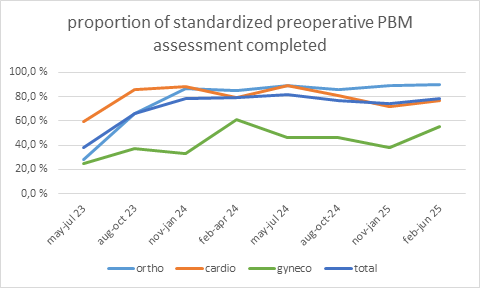
\includegraphics[width=0.9\textwidth]{figure.png}
\caption{Temporal trends of standardized preoperative PBM assessment completion rates by surgical specialty (May 2023 -- June 2025). The graph shows quarterly measurements for orthopedics (blue), cardiology (orange), gynecology (green), and overall hospital performance (dark blue).}
\label{fig:pbm_trends}
\vspace{-1em}
\end{figure}

\section{Discussion and conclusion}

The indicators show comparable dynamics across all surgical specialties, with an initial phase of growth followed by stagnation in recent periods. This could be explained by minimal clinical need—particularly for transfusion—or a lack of professional training. The latter will be addressed through microlearning modules in the coming months.

On the technical level, the current data stack is being refactored with modern tools (Dagster, dbt, OMOP) as part of a regional data warehouse initiative, enabling fully automated, web-accessible dashboards in the future.

\begin{thebibliography}{99}

\bibitem{godonReductionRedBlood2024}
Godon A, et~al. Reduction of red blood cell transfusion with a patient blood management protocol in urological and visceral surgery: a before–after study. Anaesthesia Critical Care \& Pain Medicine. 2024 Aug;43(4):101395.

\bibitem{Cance2022}
Cance C, et~al. Hypergraph based data model for complex health data exploration and its implementation in PREDIMED clinical data warehouse. Studies in Health Technology and Informatics. IOS Press; 2022.

\end{thebibliography}

\end{document}